\section{Electric Propulsion Method Selection}

To determine the baseline design for the \ac{EP} system being developed, several EP technologies were evaluated for compatibility with the requirements. Some of the primary determining factors included:

\begin{itemize}
    \item Thrust level
    \item Specific impulse
    \item Power requirements
    \item Propellant type
    \item System complexity
    \item Flight Heritage
\end{itemize}

While most of these requirements are already defined, the thrust requirement needs to be further refined.

\subsection{Thrust Requirement}
One of the reqirements was that "The system should be capable of producing a thrust level sufficient for orbit keeping of a nanosatellite at 200km altitude". To calculate the necessary thrust levels for maintaining a stable orbit at various altitudes, a python script was developed. The script considered atmospheric drag as the primary actor, while assuming all other forces such as solar radiation pressure were negligible. The drag force was calculated using the standard drag equation:

\begin{equation}
    F_d = \frac{1}{2} C_d \rho A v^2
\end{equation}
where \( F_d \) is the drag force, \( C_d \) is the drag coefficient, \( \rho \) is the atmospheric density at the given altitude, \( A \) is the cross-sectional area of the satellite, and \( v \) is the orbital velocity.

The drag coefficient \( C_d \) was assumed to be 2.2, which is typical for small satellites. (Provide a reference for this) 
The cross-sectional area \( A \) was taken as the average surface area of the satellite.
The atmospheric density \( \rho \) was estimated using the ... model, which provides values for densities of each element in the atmosphere at different altitudes.
The orbital velocity \( v \) was calculated using the formula for circular orbits:

\begin{equation}
    v = \sqrt{\frac{GM}{r}}
\end{equation}

where \( G \) is the gravitational constant, \( M \) is the mass of the Earth, and \( r \) is the distance from the center of the Earth to the satellite.


As shown in fig \ref{fig:drag_force_vs_altitude}, the script iterated over a range of altitudes and satellite sizes to compute the required thrust to counteract drag. The results were plotted to visualize the relationship between altitude, satellite size, and required thrust.

\begin{figure}[H]
    \centering
    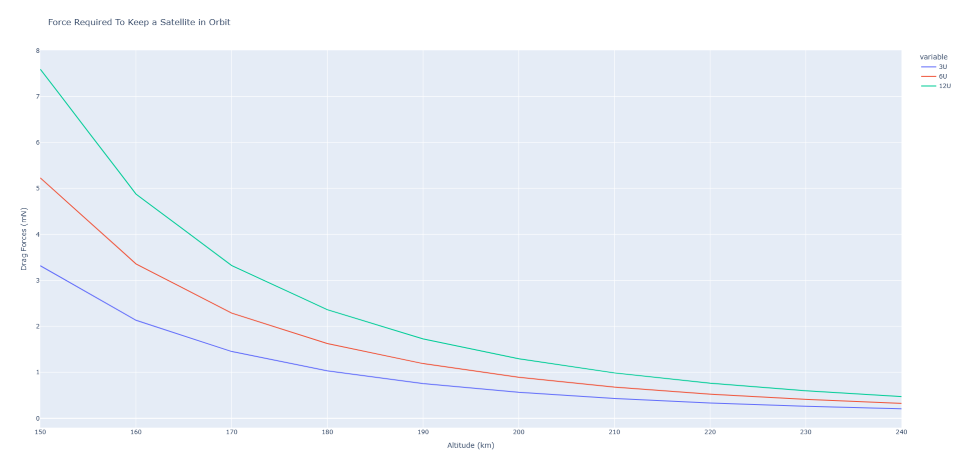
\includegraphics[width=1.0\textwidth]{images/Misc/150km - 240km.png}
    \caption{Drag Force vs Altitude for Various Satellite Sizes}
    \label{fig:drag_force_vs_altitude}
\end{figure}

Assuming that the drag force is the only force acting on the satellite, the required thrust to maintain a stable orbit is equal in magnitude and opposite in direction to the drag force. The results indicated that a thrust level of approximately ... mN would be sufficient for orbit keeping at 200km altitude for a nanosatellite in the 1-10 kg range. Hence any force greater than this would be sufficient for orbit keeping and if sufficiently higher thrust levels were available, the system could also be used for orbit raising.

\subsection{Propulsion Methods Considered}

\subsubsection{Gridded Ion Thrusters}

\subsubsection{Hall Effect Thrusters}

\subsection{Selection Results}

% Technologies such as Hall-effect thrusters, ion thrusters, and electrospray thrusters were considered.